\begin{figure}
\centering

\begin{tabular}{cc}

\begin{subfigure}[b]{0.5\textwidth}
\centering
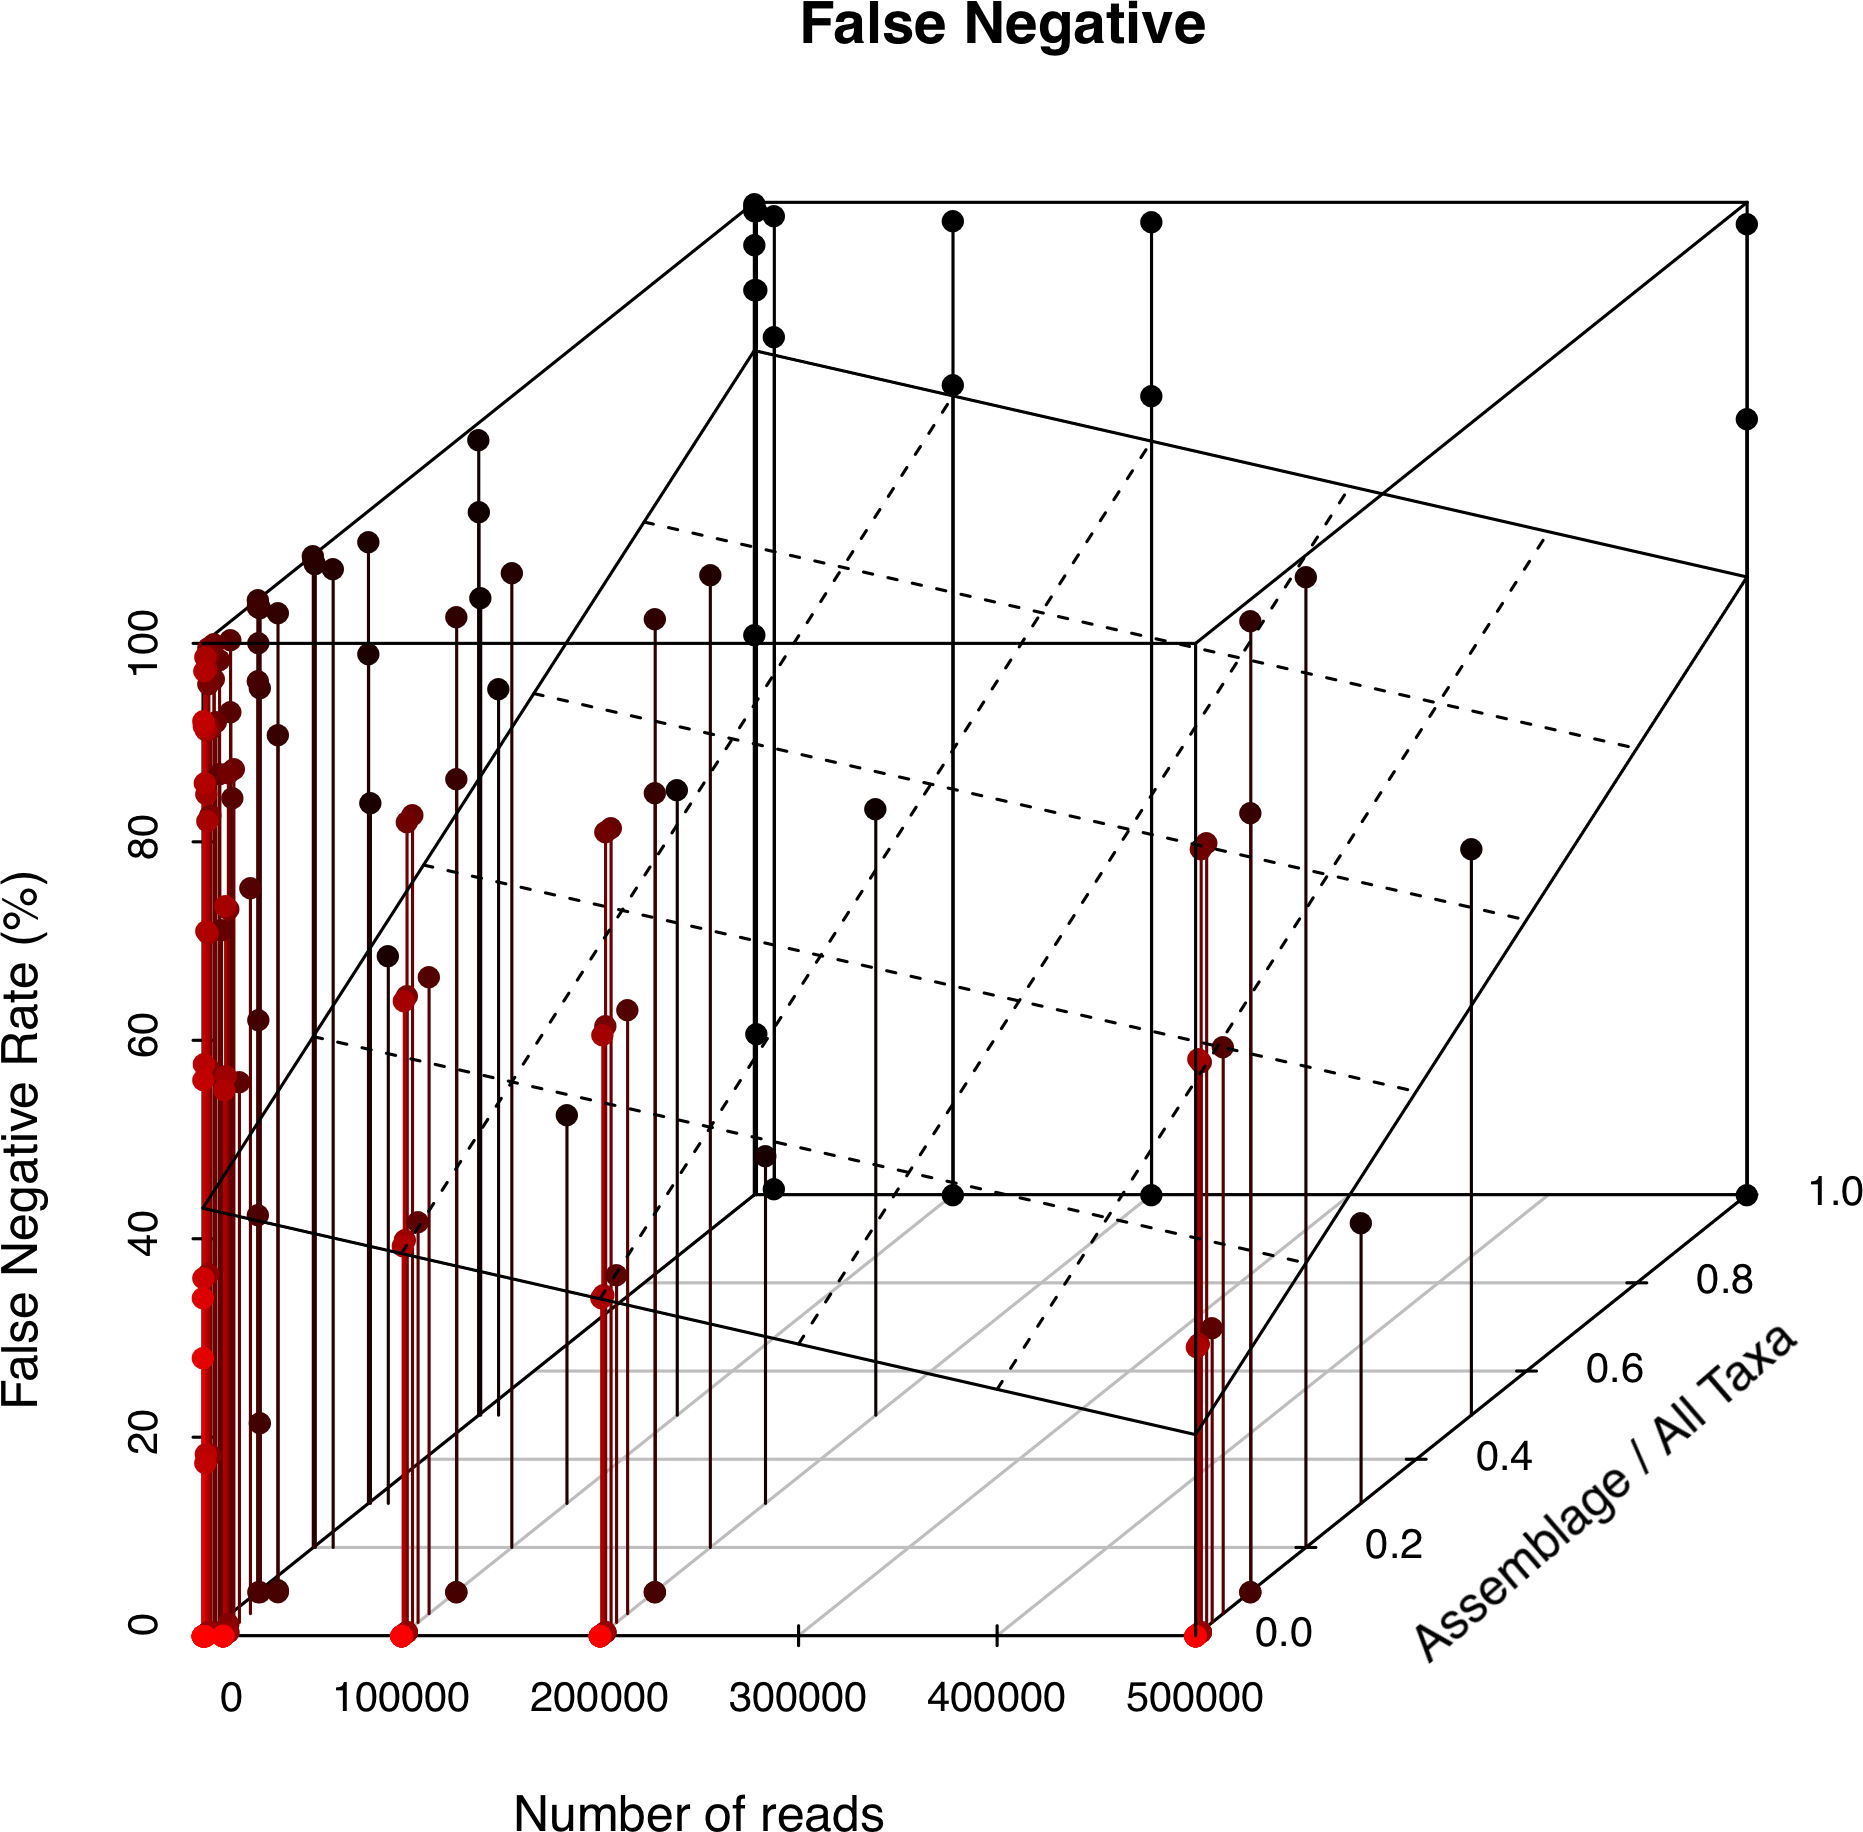
\includegraphics[width=\textwidth]{../polarfront/falsenegative.png}
\caption{False negative rate (\%) --- the percentage of taxa in the assemblage that were absent from the \softwarename{blast} results following \softwarename{minspec} processing.}
\label{fig:minspecvalidationfalsenegative}
\end{subfigure}%

&
%\quad %add desired spacing between images, e. g. ~, \quad, \qquad etc. 
%(or a blank line to force the subfigure onto a new line)

\begin{subfigure}[b]{0.5\textwidth}
\centering
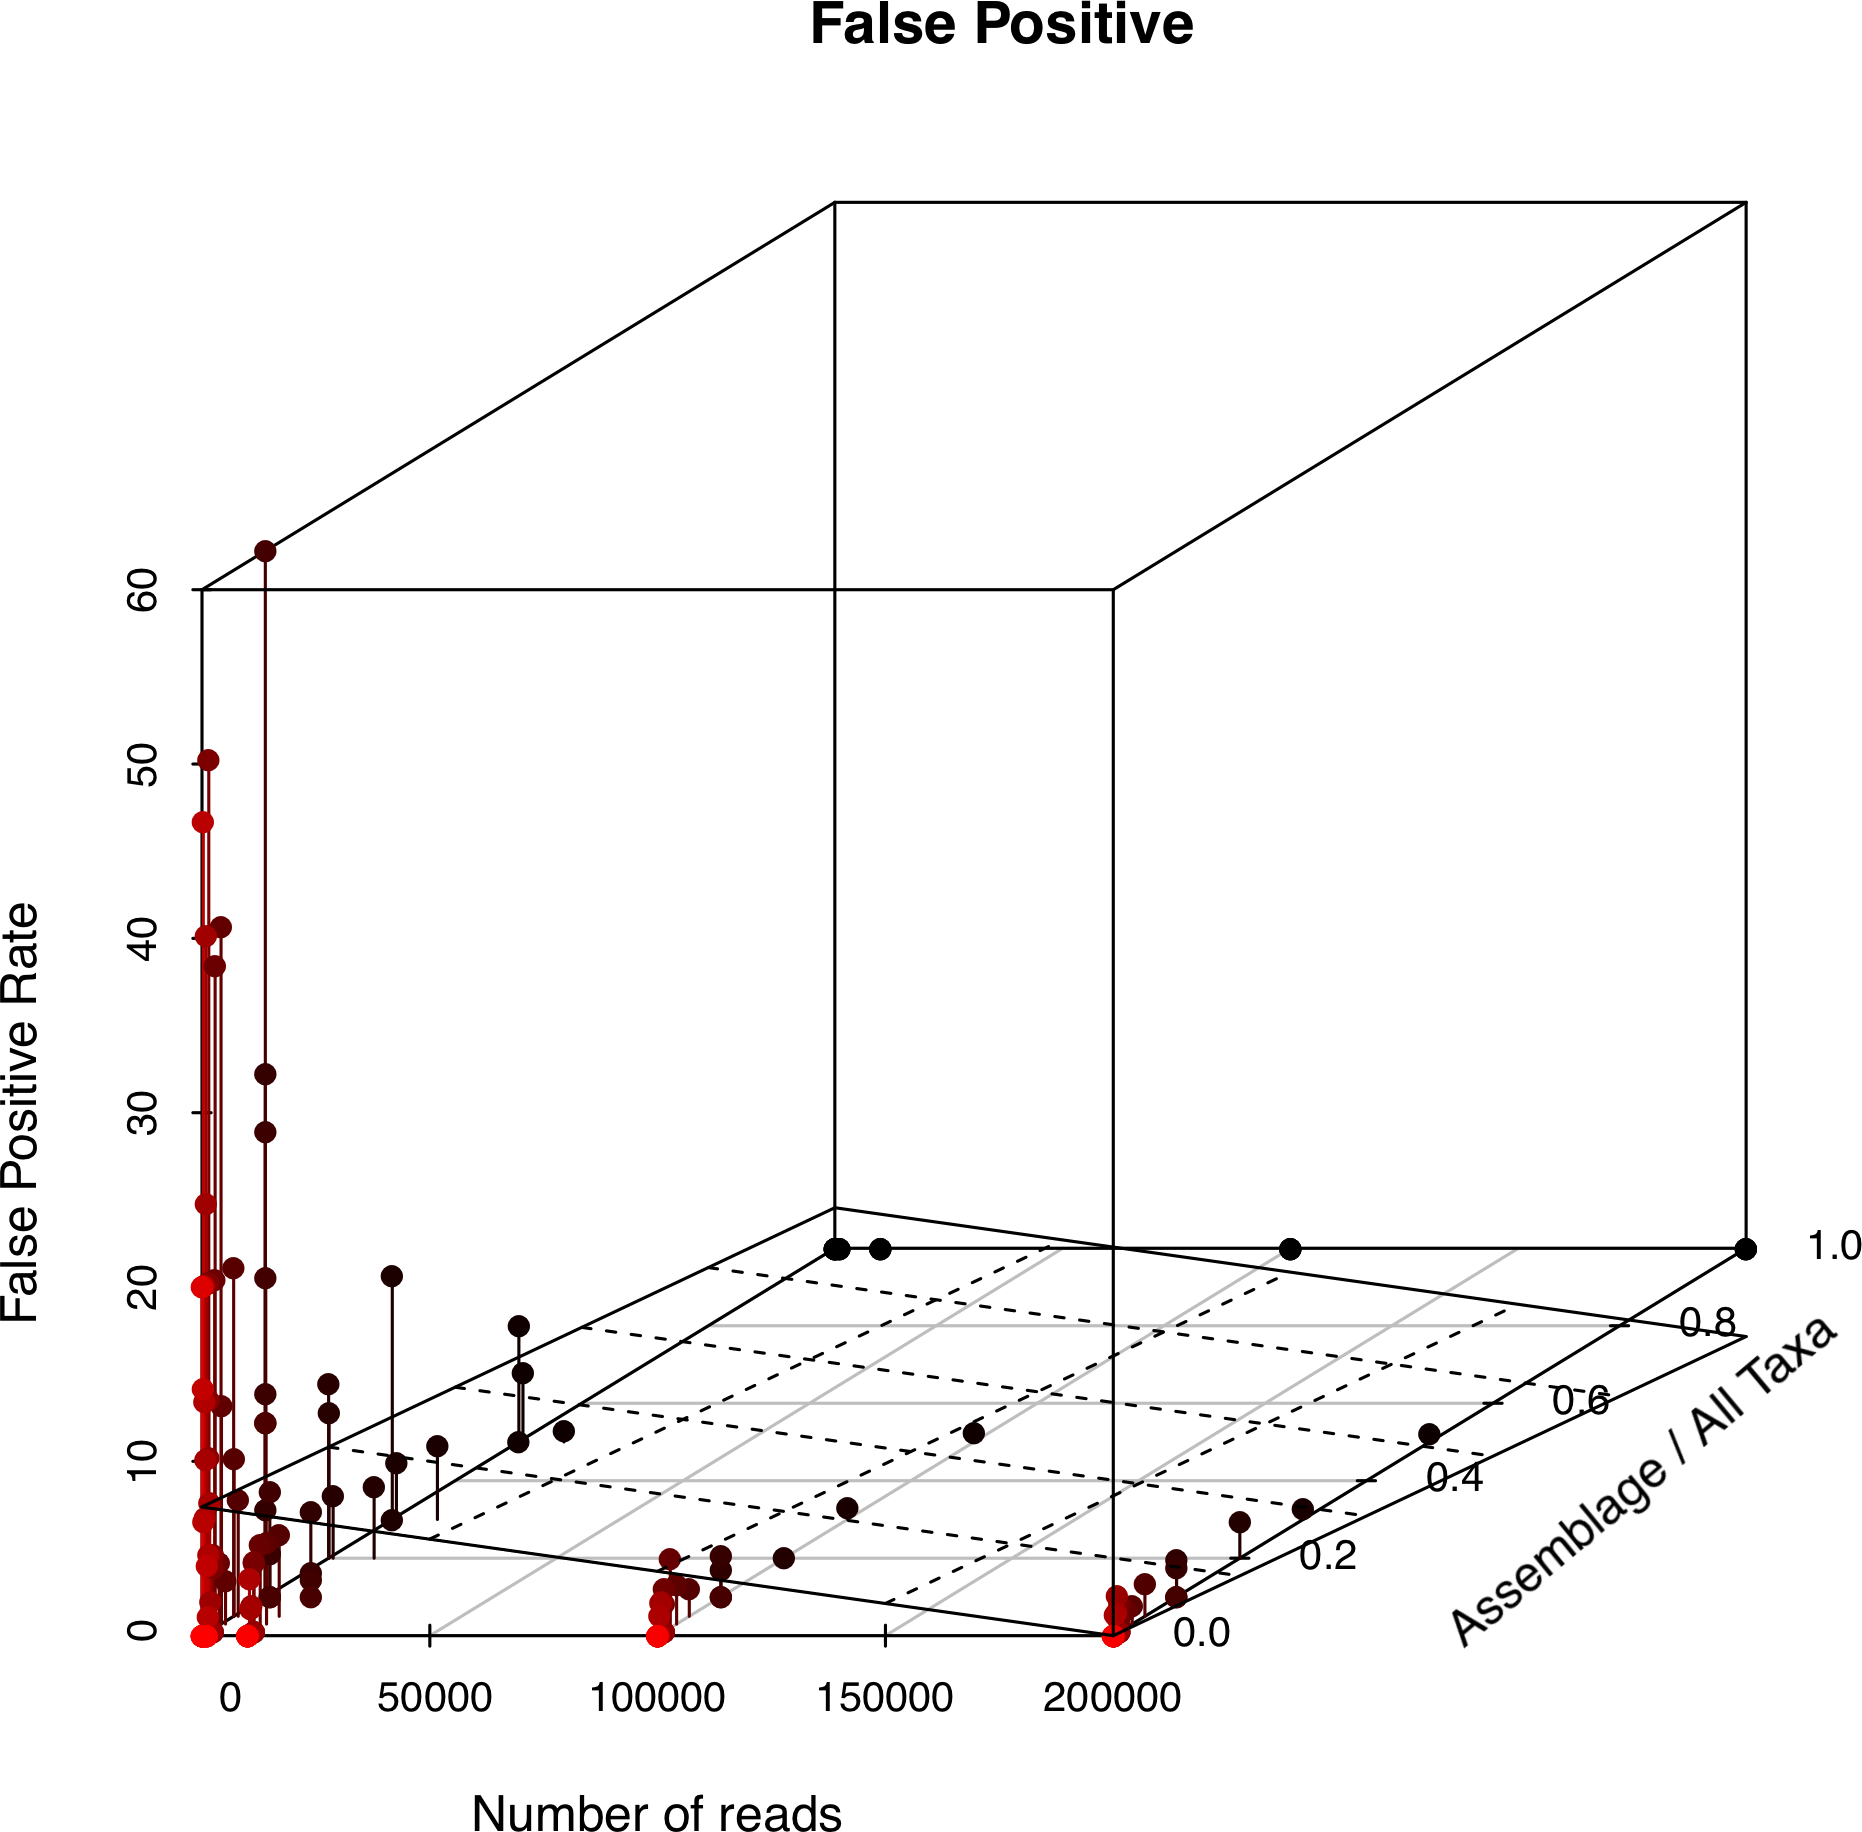
\includegraphics[width=\textwidth]{../polarfront/falsepositive.png}
\caption{False positive rate (\%) --- the percentage of taxa not in the assemblage that were present in the \softwarename{blast} results following \softwarename{minspec} processing.}
\label{fig:minspecvalidationfalsepositive}
\end{subfigure}

\bigskip
\\
\bigskip
\\
%\quad %add desired spacing between images, e. g. ~, \quad, \qquad etc. 
%(or a blank line to force the subfigure onto a new line)

\begin{subfigure}[b]{0.5\textwidth}
\centering
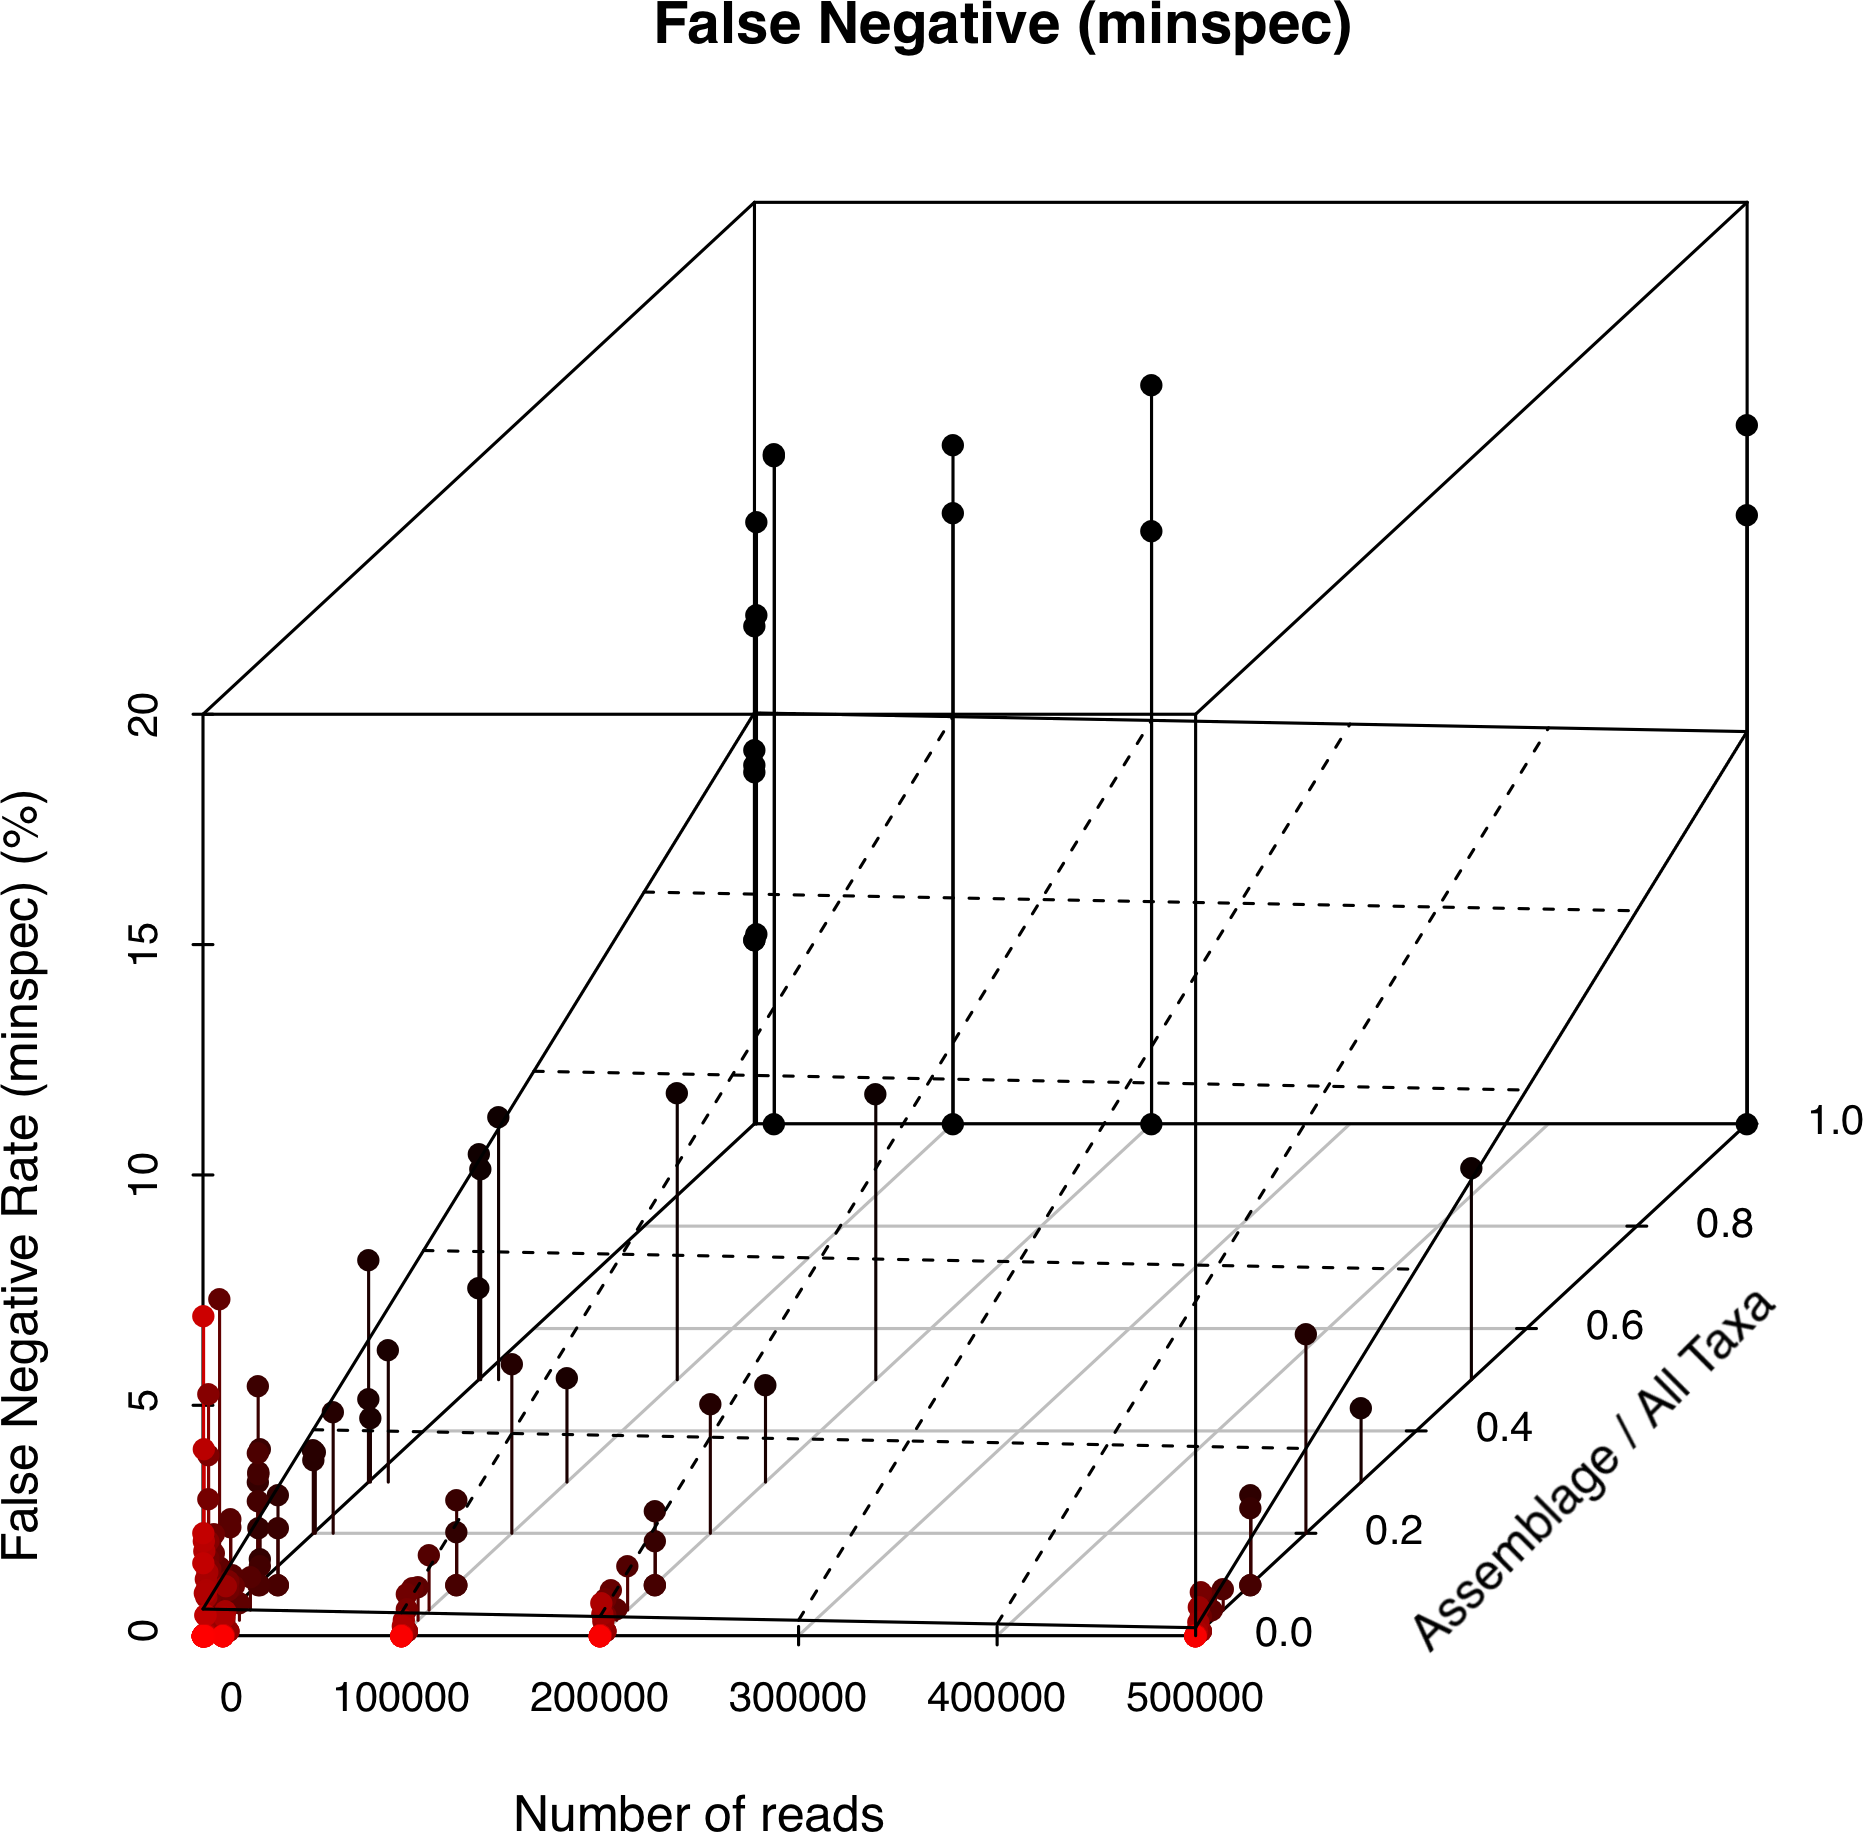
\includegraphics[width=\textwidth]{../polarfront/minspecfalsenegative.png}
\caption{\softwarename{minspec}-attributable false negative rate (\%) --- the percentage of taxa not in the assemblage that generated \softwarename{blast} hits but were incorrectly removed by \softwarename{minspec}.}
\label{fig:minspecvalidationminspecfalsenegative}
\end{subfigure}

&
%\quad %add desired spacing between images, e. g. ~, \quad, \qquad etc. 
%(or a blank line to force the subfigure onto a new line)

\begin{subfigure}[b]{0.5\textwidth}
\centering
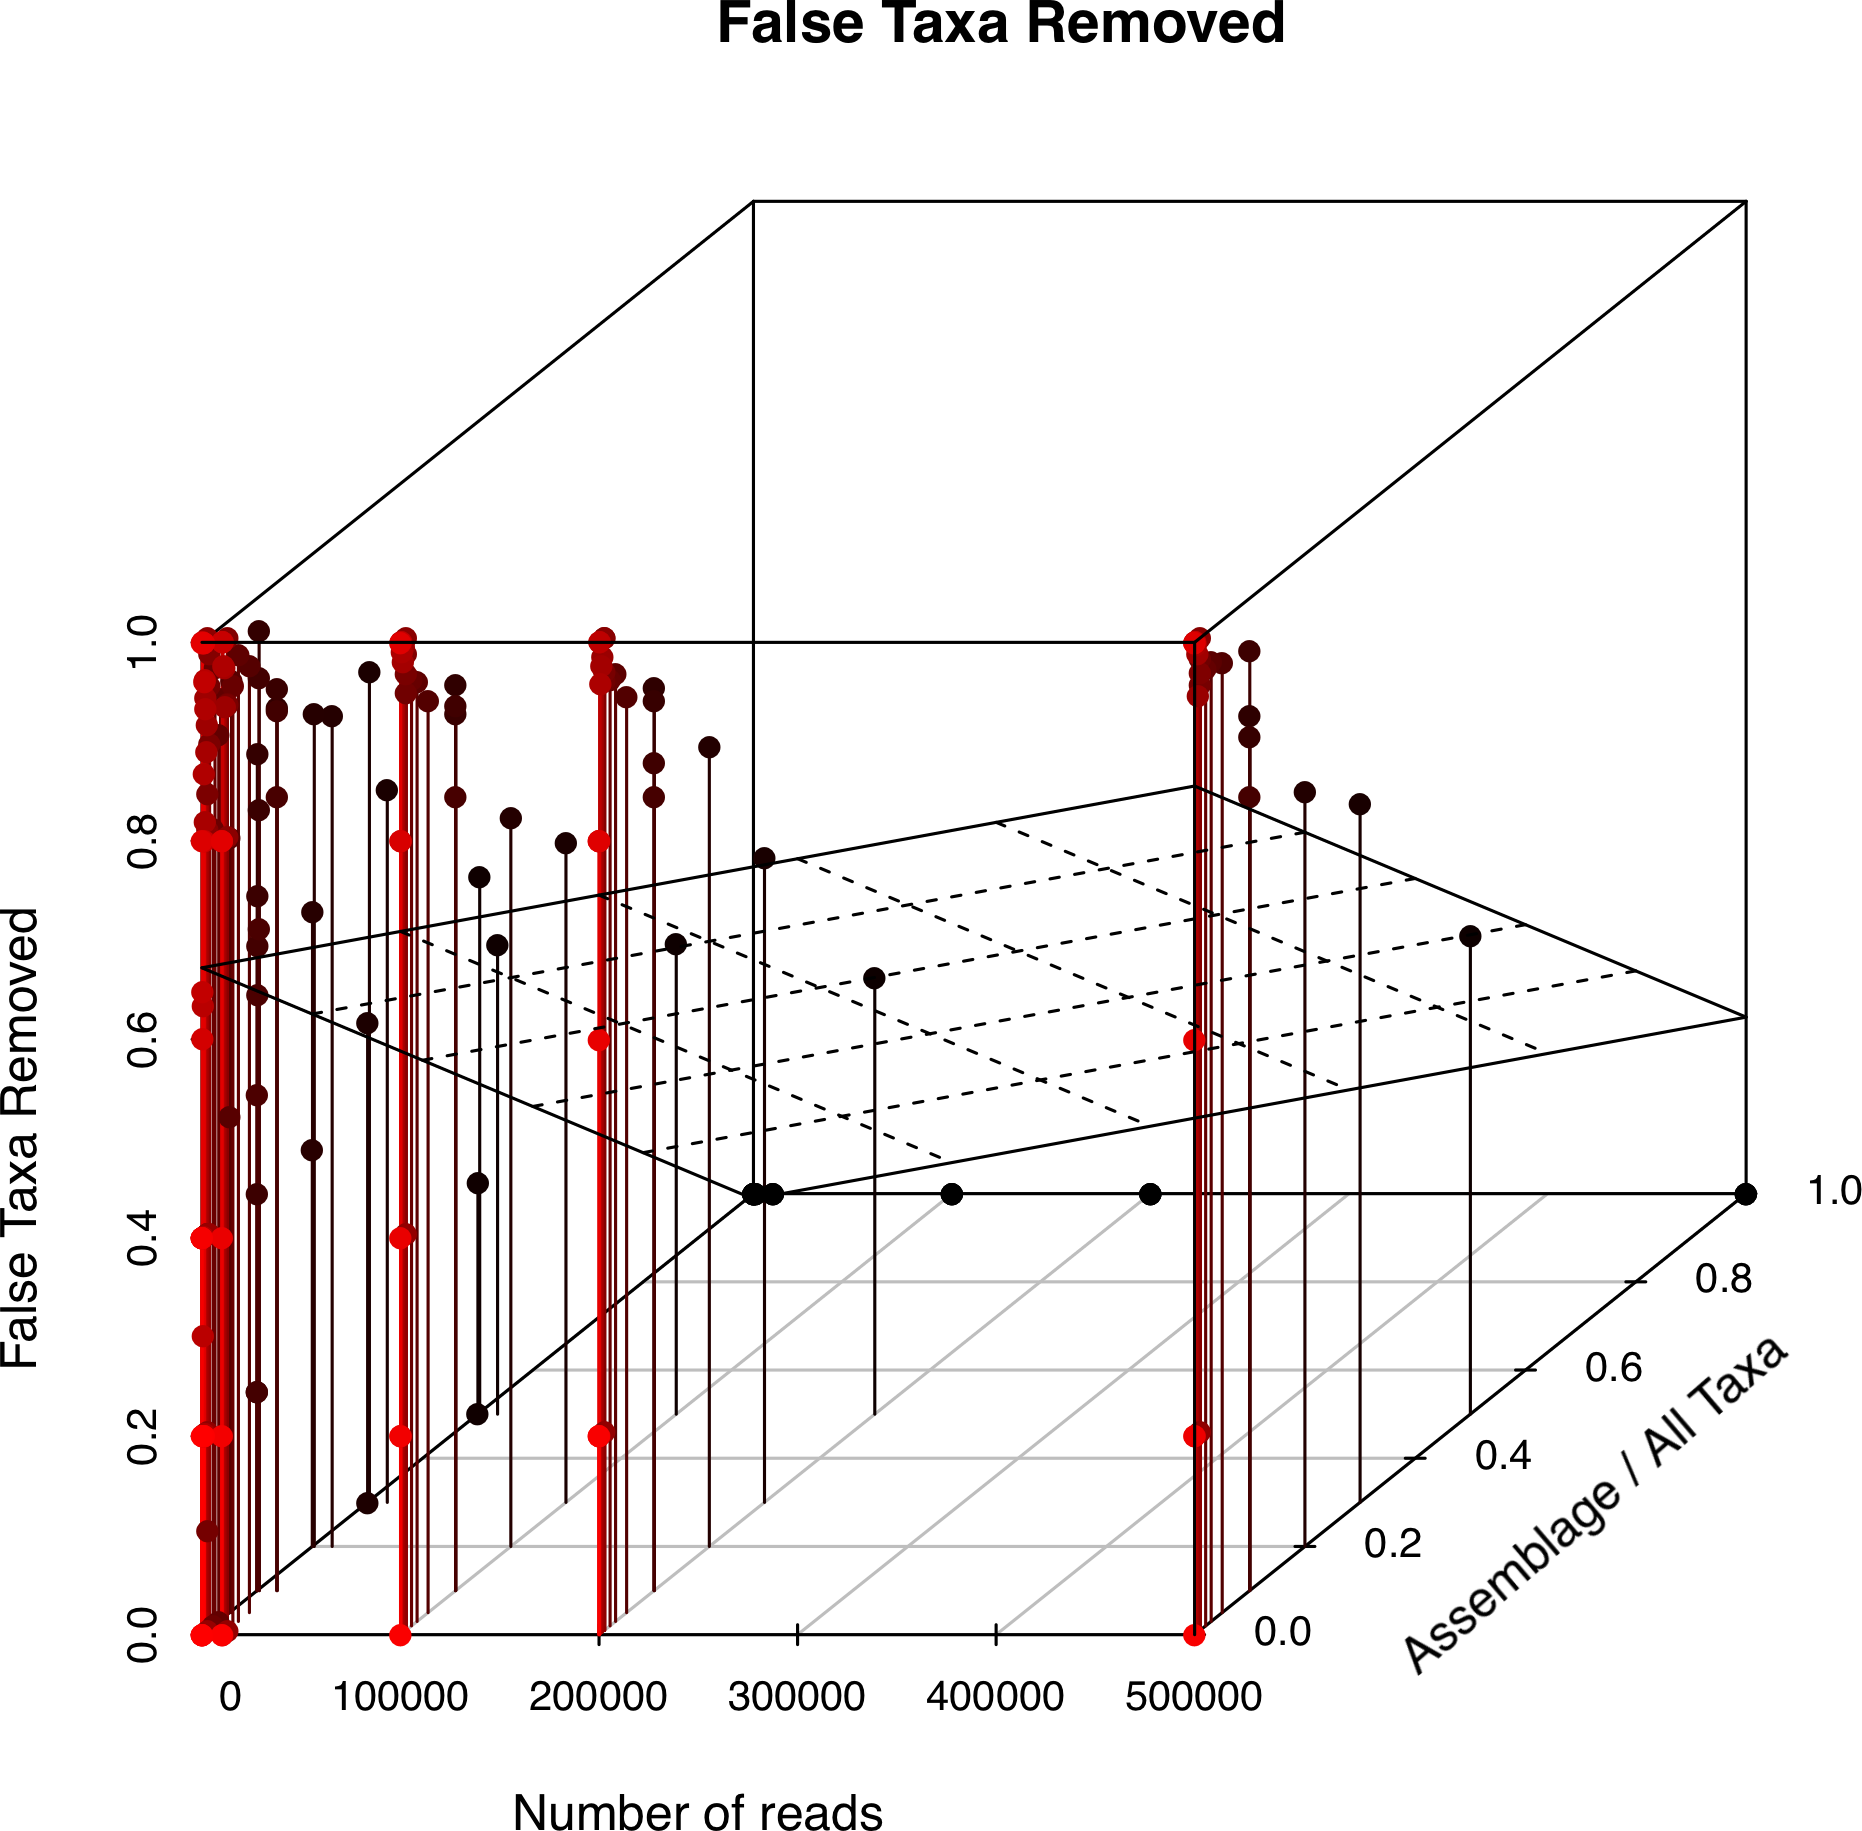
\includegraphics[width=\textwidth]{../polarfront/falsetaxaremoved.png}
\caption{Proportion of false taxa --- taxa that were not part of the simulated assemblage but which generated hits due to simulated sequence identity --- that were correctly identified and removed by \softwarename{minspec}.}
\label{fig:minspecvalidationfalsetaxaremoved}
\end{subfigure}
\\

\end{tabular}

\caption[Results of \softwarename{minspec} validate]{Results of repeated trials of \softwarename{minspec} on simulated metagenomic studies with multiple permutations of parameters (number of reads, number of simulated taxa, size of simulated assemblage).
The number of simulated taxa and size of simulated assemblage are representated as a ratio on the z-axis (``assemblage / all taxa'').
Each permutation was repeated five times.
A plane representing a linear regression has been overlayed on each plot to indicate the trend.
Points have been tinted to aid the perception of depth.
}\label{fig:minspecvalidation}
\end{figure}
